\documentclass[a4paper,
  10pt,
  english,
  DIV=12,
  BCOR=8mm]{scrbook}
\usepackage[utf8x]{inputenc}
\usepackage{babel}
\usepackage{listings}
\usepackage{xcolor}
\usepackage{hyperref}
\usepackage{siunitx}
\usepackage[T1]{fontenc}
\usepackage{isodate}
\usepackage{graphicx}
\usepackage{amsthm}
\usepackage{acronym}
\usepackage{amssymb}
\usepackage{tikz}
\usepackage{pgfplots}
\usepackage{caption}
\usepackage{subcaption}
\usepackage{booktabs}
\usepackage{xspace}
\usepackage{overpic}

\DeclareSIUnit\byte{B}
\DeclareSIUnit\basepairs{bp}
\DeclareSIUnit\bit{bit}

\definecolor{oceangreen}{cmyk}{1,.0,.20,.78}
\addtokomafont{sectioning}{\rmfamily\color{oceangreen}}

\definecolor{bluekeywords}{rgb}{0.13,0.13,1}
\definecolor{greencomments}{rgb}{0,0.5,0}
\definecolor{turqusnumbers}{rgb}{0.17,0.57,0.69}
\definecolor{redstrings}{rgb}{0.5,0,0}
\definecolor{lightgray}{rgb}{0.9,0.9,0.9}

\usepackage{libertine}
\fontfamily{libertine}
\selectfont
%\usepackage[scaled]{berasans}

\newcommand{\thymine}{\textsc{m}\oldstylenums{2}\xspace}
\newcommand{\local}{\textsc{m}\oldstylenums{1}\xspace}
\newcommand{\algo}[1]{\textsc{{#1}}}
\newcommand{\andi}{\algo{andi} }
\newcommand{\word}[1]{\textsf{\small#1}}
\newcommand{\wchar}[1]{\textsf{\small#1}}
\newcommand{\eco}{\textsc{eco}\oldstylenums{29}\xspace}
\newcommand{\pneu}{\textsc{Pneu}\oldstylenums{3085}\xspace}

% Todos at the margin
\newcommand{\todo}[1]{
  \marginpar{\fbox{\begin{minipage}{0.9\marginparwidth}
  \scriptsize\sloppy\raggedright #1
  \end{minipage}}}
}


\newtheorem{definition}{Definition}


\lstset{backgroundcolor=\color{lightgray}}

\lstdefinestyle{shell}{
	language=bash,
	columns=flexible,
  xleftmargin=12pt,
  xrightmargin=12pt,
  breaklines=true,
  basicstyle=\small\ttfamily,
  morekeywords={make, tar, git, sudo, andi, time, man, head, cut, fneighbor, fretree, figtree},
 % literate={~} {$\sim$}{1}
}


\lstdefinelanguage{algo}{
  sensitive=true,
  classoffset=0,
  keywords={let,while,end,if,then,else,output,input,do,fn,requires,and,or,continue,to,for, goto, line, of, number, array, each, true, false, break, match},
  keywordstyle=\color{bluekeywords},
  classoffset=0,
  string=[b]{'},
  stringstyle={\color{greencomments}},
  morecomment=[l][\color{greencomments}]{//},
  literate={->}{{$\to$ }}{1}{\{}{{$\{$}}{1}{\}}{{$\}$}}{1}{!D}{{\$}}{1}{<-}{{$\leftarrow$ }}{1}{sigma}{{$\sigma$}}{1}
}

\lstdefinestyle{algo}{
  language=algo,
  mathescape=true,
  columns=flexible,
  identifierstyle=\emph,
  inputencoding=utf8x,
  tabsize=4,
  escapeinside={(*}{*)},
  numbers=left,
  xleftmargin=2em,
  numberstyle=\scriptsize,
}

\lstset{style=shell}

\title{\algo{andi}: the anchor distance}
\subtitle{Efficient Alignment-Free Estimation of Evolutionary Distances\\ {\small\url{https://github.com/EvolBioInf/andi}}}
\author{Fabian Klötzl\\ \href{mailto:kloetzl@evolbio.mpg.de}{kloetzl@evolbio.mpg.de}}
\date{Version 0.9, \isodate\today \\
\vspace*{2cm}
\centering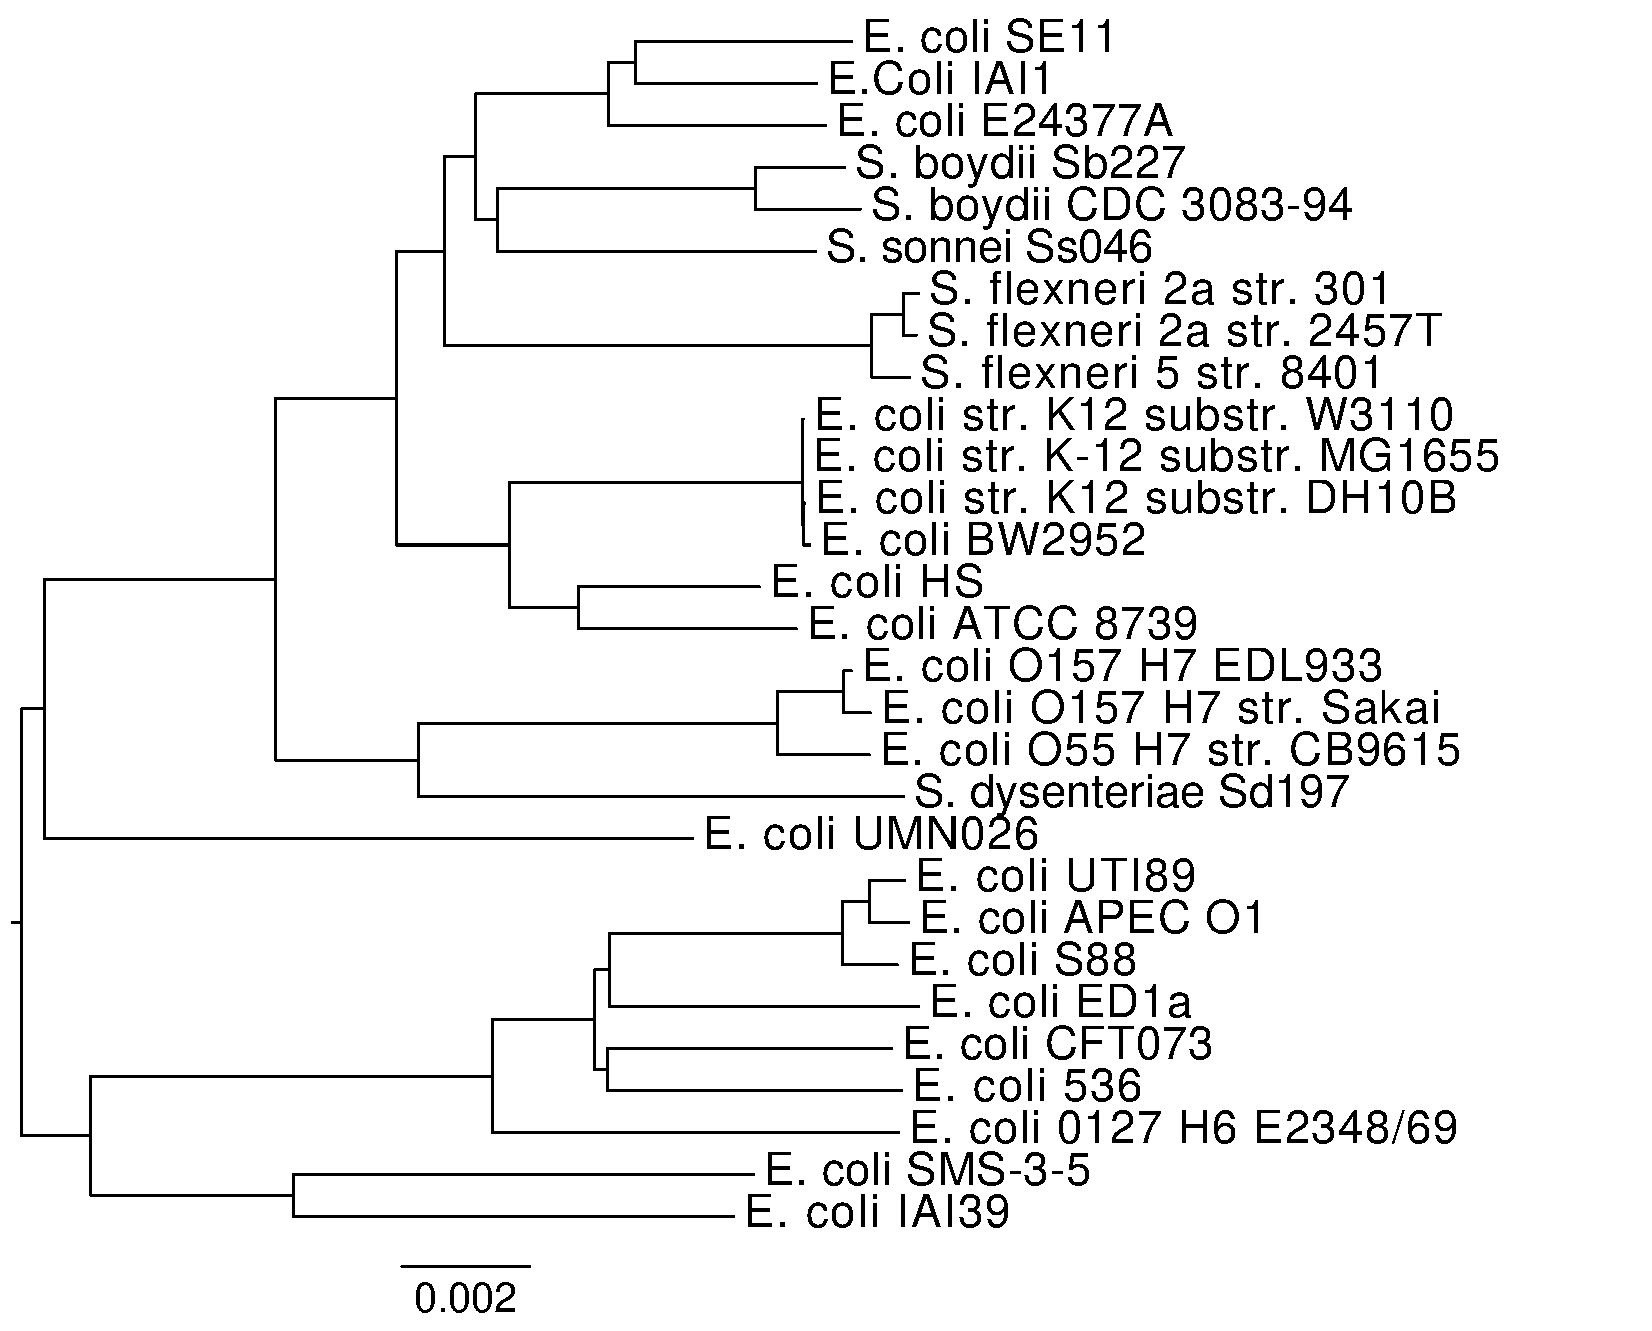
\includegraphics[width=0.8\textwidth]{img/eco29/andi_labels.pdf}}

\begin{document}

\maketitle

\section*{Abstract}
%\begin{abstract}
  This is the documentation of the \andi program for estimating the evolutionary distance between closely related genomes. It efficiently and accurately computes a distance for substitution rates up to 0.5. These distances are based on ungapped local alignments framed by anchors. Anchors are efficiently found using an enhanced suffix array. As a result, \andi scales well, even for data sets containing thousands of bacterial genomes.
%\end{abstract}

\vspace*{1cm}
\section*{License}
This document is release under the Creative Commons Attribution Share-Alike license. This means, your are free to copy and redistribute this document. You may even remix, tweak and build upon this document, as long as you credit me for the work I've done and release your document under the identical terms. The full legal code is available online: {\small\url{https://creativecommons.org/licenses/by-sa/4.0/legalcode}}.

\tableofcontents

\chapter{Installation} %%%%%

The easiest way to obtain your own copy of \algo{andi}, is to download the latest release from GitHub.\footnote{\url{https://github.com/EvolBioInf/andi/releases}} Please note, that \andi requires \algo{libdivsufsort}\footnote{\url{https://github.com/y-256/libdivsufsort}} for optimal performance. If you wish to install \andi without \algo{libdivsufsort}, consult Section~\ref{sub:wo-divsufsort}.

\section{Installing from Source Package} \label{sub:regular}

Once you have downloaded the package, unzip it and change into the newly created directory. 

\begin{lstlisting}
~ %  tar -xzvf andi-0.9.tar.gz
~ %  cd andi-0.9
\end{lstlisting}

\noindent You should now see plenty of files, of which most better stay untouched. If you feel that this documentation is too verbose, and you prefer more succinct instructions, please consult the \lstinline$README$. However, if you are still reading this, execute the following commands, to proceed.

\begin{lstlisting}
~/andi-0.9 %  ./configure
~/andi-0.9 %  make
~/andi-0.9 %  sudo make install
\end{lstlisting}

\noindent This installs \andi for all users on your system. If you do not have root privileges, you will find a working copy of \andi in the \lstinline$src$ subdirectory. For the rest of this documentation, I will assume, that \andi is in your \textdollar\lstinline!PATH!.

Now \andi should be ready for use. Try invoking the help.

\begin{lstlisting}
~/andi-0.9 %  andi -h
Usage: andi [-jrv] [-p FLOAT] FILES...
	FILES... can be any sequence of FASTA files. If no files are supplied, stdin is used instead.
Options:
  -j, --join        Treat all sequences from one file as a single genome
  -m, --low-memory  Use less memory at the cost of speed
  -p <FLOAT>        Significance of an anchor pair; default: 0.05
  -r, --raw         Calculates raw distances; default: Jukes-Cantor corrected
  -v, --verbose     Prints additional information
  -t <INT>          The number of threads to be used; default: 1
  -h, --help        Display this help and exit
      --version     Output version information and acknowledgments
\end{lstlisting}

\noindent \andi also comes with a man page, which can be accessed via \lstinline$man andi$. But once you are done with this documentation, you will require it scarcely.

\section{Installing without \algo{libdivsufsort}} \label{sub:wo-divsufsort}

If you cannot or do not want to install \algo{libdivsufsort}, \andi has got you covered. It comes with its own implementation for a \emph{suffix array construction algorithm}. That one is called \algo{psufsort} and features its own \algo{Git} repo.\footnote{\url{https://github.com/kloetzl/psufsort}} To activate it for \algo{andi}, proceed as described in Section~\ref{sub:regular}, but with the following twist:

\begin{lstlisting}
~/andi %  ./configure --without-libdivsufsort
\end{lstlisting}

Please note that this requires a C++11 compiler. Also, \algo{psufsort} may be slower than \algo{libdivsufsort} and thus lead to inferior runtimes.

\section{Installing from Git Repository}

To build \andi from the \algo{Git} repo, execute the following steps.

\begin{lstlisting}
~ %  git clone git@github.com:EvolBioInf/andi.git
~ %  cd andi
~/andi %  autoreconf -i
\end{lstlisting}

\noindent For old versions of \algo{autoconf} you may instead have to use \lstinline$autoreconf -i -Im4$.

\noindent Continue with the \algo{Gnu} trinity as in Section~\ref{sub:regular}.


\chapter{Usage} %%%%%

The input sequences for \andi should be in \algo{Fasta} format. Any number of files can be passed. Each file can contain more than one sequence.

\begin{lstlisting}
~ %  andi S1.fasta S2.fasta
2
S1        0.0000 0.0979
S2        0.0979 0.0000
\end{lstlisting}

If no file argument is given, \andi reads the input from \algo{stdin}. This makes it convenient to use in \algo{Unix} pipelines.

\begin{lstlisting}
~ %  cat S1.fasta S2.fasta | andi
2
S1        0.0000 0.0979
S2        0.0979 0.0000
\end{lstlisting}

The output of \andi is a matrix in \algo{Phylip} style: On the first line, the number of compared sequences is given. Then the matrix is printed, where each line is proceeded by the name of the $i$th sequence. Note that the matrix is symmetric and the main diagonal contains only zeros. The numbers themselves are evolutionary distances, estimates as substitution rates.


\section{Input} \label{sec:join}

As mentioned before, \andi reads in \algo{Fasta} files. It recognizes only the four standard bases, case insensitive (\lstinline![acgtACGT]!). All other nucleotides are excluded from the analysis and \andi prints a warning, when this happens.

Today, a lot of genome projects to not end with complete genomes; instead short contigs for the genomes are given. If all contigs of a genome are in a single \algo{Fasta} file, \andi will treat them as belonging together, when switched to \algo{join} mode. This can be achieved by using the \lstinline!-j! or \lstinline!--join! command line switch.

\begin{lstlisting}
~ %  andi --join E_coli.fasta Shigella.fasta
[Output]
\end{lstlisting}

When the \algo{join} mode is active, the file names are used to name the individual sequences. Thus, in \algo{join} mode, each genomes has to be in its own file, and furthermore, at least one filename has to be given via the command line.

If \andi seems to take unusually long, or requires huge amounts of memory, then you might have forgotten the \algo{join} switch. This makes \andi compare each contig instead of each genome, resulting in much more comparisons! To make \andi output the number of genome it wants to compare use the \lstinline$--verbose$ switch.

\section{Output}

The output of \andi is written to \lstinline$stdout$. This makes it easy to use on the command line and within shell scripts. As seen before, the matrix, computed by \algo{andi}, is given in \algo{Phylip} format.

\begin{lstlisting}
~ %  cat S1.fasta S2.fasta | andi
2
S1        0.0000 0.0979
S2        0.0979 0.0000
\end{lstlisting}

If the computation completed successful, \andi exits with the status code 0. Otherwise, the \lstinline$errno$ is used as the exit code. \andi can also produce a lot of warnings and error messages for the users convenience. These messages are printed to \lstinline$stderr$ and thus do not interfere with the normal output. Please consult your shells manual for redirection of streams.

\section{Options}

\andi takes a small number of commandline options, of which even fewer are of interest on a day-to-day basis. If \lstinline$andi -h$ displays a \lstinline$-t$ option, then \andi was compiled with multi-threading support (implemented using \algo{OpenMP}). By default \andi uses all available processors. However, if you want to restrict the number of threads use \lstinline$-t$.

\begin{lstlisting}
~ %  time andi ../test/1M.1.fasta -t 1
2
S1        0.0000 0.0995
S2        0.0995 0.0000
./andi ../test/1M.1.fasta  0,60s user 0,01s system 99% cpu 0,613 total
~ %  time andi ../test/1M.1.fasta -t 2
2
S1        0.0000 0.0995
S2        0.0995 0.0000
./andi ../test/1M.1.fasta -t 2  0,67s user 0,03s system 195% cpu 0,362 total
\end{lstlisting}

Note that in the above examples the runtime reduced from \SI{0.613}{\second}, to \SI{0.362}{\second} using two threads. Making \andi use more threads than input genomes leads to no further speed improvement.

The other most-important option is \lstinline$--join$. It is used, when the genomes consist of multiple contigs. For more information, see section~\ref{sec:join}.

By default, the distances computed by \andi are \emph{Jukes-Cantor} corrected. This means, the output is substitution rates, which is slightly larger than the mismatch rate. If you want to calculate the pure mismatch rate, \andi can do so if told so by the \lstinline$--raw$ switch.

% If you are using very big data sets whose size is close to your machines RAM you may find \andi becoming slow because of swapping or even dying from memory shortage. In these cases you can switch \andi into a \emph{low-memory} mode. Note: this only helps for multithreading

\section{Example: \algo{eco29}}

Here is a simple real-world example on how to use \algo{andi}. As a data set we'll be using \algo{eco29}; 29 genomes of \textit{E. Coli} and \textit{Shigella}. You can download the data here: {\small{\url{http://guanine.evolbio.mpg.de/andi/eco29.fasta.gz}}}. The genomes have an average length of 4.9~million nucleotides amounting to a total \SI{138}{\mega\byte}.

\algo{eco29} comes a single \algo{fasta} file, where each sequence is a genome. Applying \andi to this data set is straightforward.

\begin{lstlisting}
~ % andi eco29.fasta > eco29.mat
andi: The input sequences contained characters other than acgtACGT. These were automatically stripped to ensure correct results.
\end{lstlisting}

\noindent The \algo{eco29} data set includes non-canonical nucleotides, such as \word{Y}, \word{N}, and \word{P}. Unfortunately, \andi cannot process these, thus they get stripped from the input sequences. The resulting matrix is stored in \lstinline$eco29.mat$. Because the complete matrix would be too big for this page, here is a small excerpt.

\begin{lstlisting}
~ % head -n 5 eco29.mat | cut -d ' ' -f 1-5
29
gi|563845 0.0000e+00 1.8388e-02 1.8439e-02 2.6398e-02
gi|342360 1.8388e-02 0.0000e+00 4.4029e-04 2.6166e-02
gi|300439 1.8439e-02 4.4029e-04 0.0000e+00 2.6123e-02
gi|261117 2.6398e-02 2.6166e-02 2.6123e-02 0.0000e+00
\end{lstlisting}

\noindent From this we now have to compute a tree via neighbor-joining. For this, I use a wrapper of \algo{Phylip} called \algo{Embassy}.\footnote{\url{http://emboss.sourceforge.net/embassy/\#PHYLIP}} Because I enjoy rooted phylograms, I also midpoint-root the tree.

\begin{lstlisting}
~ % fneighbor -datafile eco29.mat -outfile eco29.phylipdump
~ % fretree -spp 29 -intreefile eco29.treefile -outtreefile eco29.tree <<EOF
M
X
Y
R
EOF
\end{lstlisting}

\noindent The file \lstinline$eco29.tree$ now contains the tree in Newick format. Finally, the resulting phylogeny can be plotted using any tool of your choice. 

\begin{lstlisting}
~ % figtree eco29.tree &
\end{lstlisting}

\noindent Here is the tree I computed. Yours should look similar.

\begin{figure}[h]
  \centering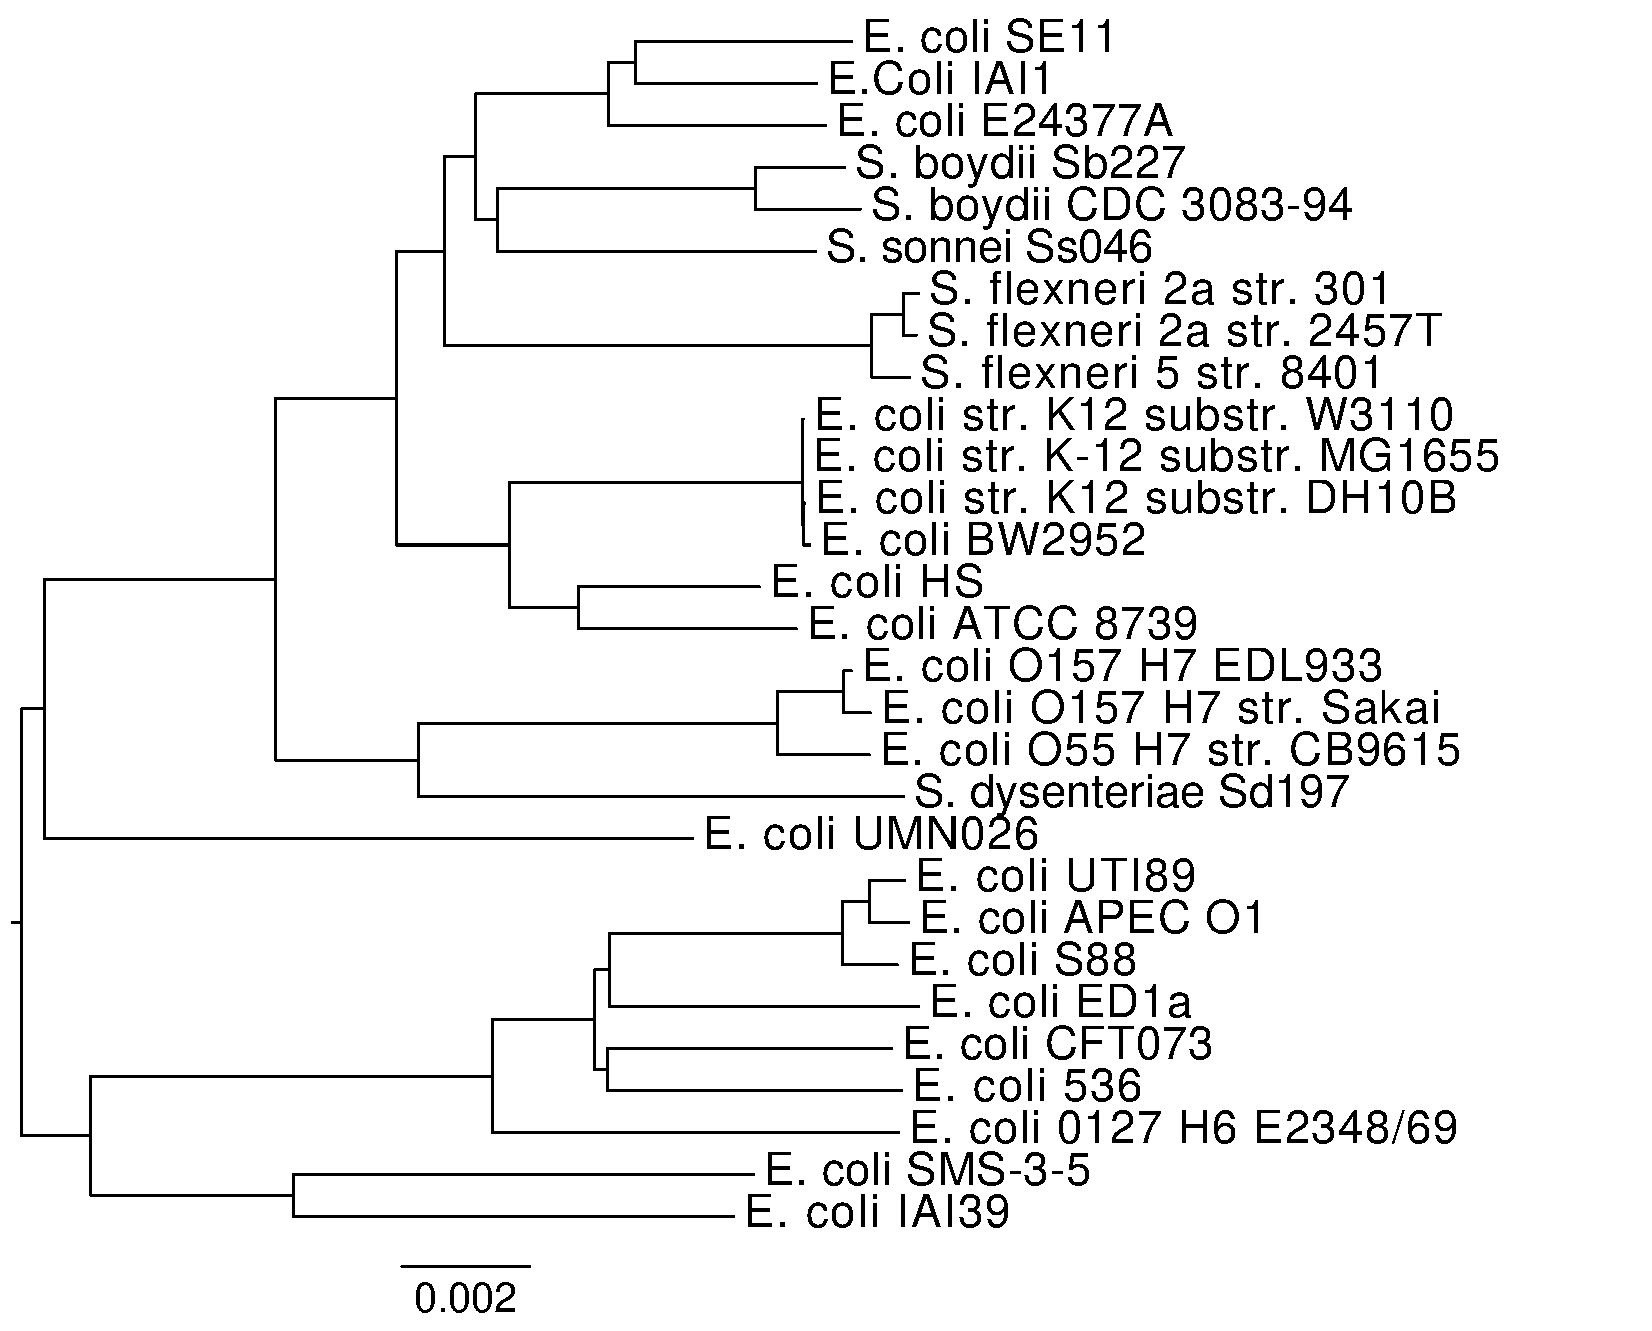
\includegraphics[width=0.8\textwidth]{img/eco29/andi_labels.pdf}
\end{figure}


\chapter{The Anchor Distance in Detail}

This section explains the idea of the \emph{anchor distance}. After doing this in detail, we also compare this process with other \emph{alignment-free} tools and verify the results with reference alignments. Parts of this section come from my master thesis which I will provide at request.

\section{Motivation}

Computing a phylogeny is a standard task arising in the analysis of genomes. There are various approaches to compute such a phylogeny. Often, this is done by computing an (multiple) alignment and then creating a matrix of evolutionary distances.

% Alignment

\noindent Interestingly, when the evolutionary distances are calculated from an alignment, indels are usually ignored. This means, the time which was spent on computing gaps is a waste of effort. If instead one can estimate the substitution rate directly from the data, the resulting pipeline will be much faster. This is essentially the idea of most \emph{alignment-free} distance estimators.

\section{Definition}

The anchor distance is computed from two sequences, one called the \emph{subject} $S$ and a \emph{query} $Q$ with $Q,S \in \{A,C,G,T\}^*$\footnote{Even though the genomic alphabet contains only the four characters $A,C,G$ and $T$, the actual alphabet used by \algo{andi} has the following additional characters $\{!, ;, \#, \backslash 0 \}$. The $\#$ is used to separate a genome sequence from its reverse complement. Both of which might be made up of multiple contigs separated by $!$ and $;$, respectively.}. Due to evolutionary events like \emph{gene duplication}, the comparison with our yet-to-be-defined anchor distance $d_\mathit{asym}$ may not be symmetric (i.\,e.,\ $d_\mathit{asym}(Q,S) \ne d_\mathit{asym}(S,Q)$). To overcome this limitation, the final distance is the average of both comparisons.


\begin{definition}[Anchor Distance] Let $S_1$ and $S_2$ be two genetic sequences. Then the \emph{anchor distance} is the average of the two asymmetric comparisons with $d_\mathit{asym}$.
\[
  d_a(S_1, S_2) = \frac{d_\mathit{asym}(S_1,S_2)+d_\mathit{asym}(S_2,S_1)}{2}
\]
\end{definition}

To compute the asymmetric anchor distance of $S$ and $Q$, generate the \ac{ESA} of the subject, concatenated with its \emph{reverse complement}. Then $Q$ is streamed against $S$ as follows. Set $q$ to $0$ and continue until it runs past $|Q|$. Compute the longest match of $Q[q..]$ with $S$. Continue finding matches and each time incrementing $q$ by the length of the match until an anchor is found.

\begin{definition}[Anchor]
  Let $Q[q..]$ be a match which cannot be further extended to the right. If it is unique in $S$ and of some minimal length $L$, it is termed an \emph{anchor}.
\end{definition}

Save the characteristics of the first anchor and keep finding matches until a second anchor is found. Unless the anchors form an \emph{anchor pair}, replace the saved state of the first anchor with the second and try finding another second anchor. The anchors form a pair if they are equidistant, that is, their distance on $Q$ is the same as for their counterparts on $S$ (see Figure~\ref{fig:anchor_pair}).

\begin{figure}
  \centering
  \begin{tikzpicture}[every node/.style={
    rectangle,
    %draw,
    minimum height=0.1cm,
    minimum width=0.1cm,
  }, shorten >= 2pt, shorten <= 2pt]

  \node (n0) {$Q$};
  \node[right of=n0, minimum width=1cm, draw=white, node distance=2cm, fill=green!25] (n1) {};
  \node[right of=n1, minimum width=1cm, draw=white, node distance=1.5cm, fill=blue!25] (n2) {};
  \node[right of=n2] (n3) {};

  \draw (n0) -- (n1);
  \draw (n1) edge[draw=red] (n2);
  \draw (n2) -- (n3);

  \node[right of=n3] (n4) {$S$};
  \node[right of=n4, minimum width=1cm, draw=white, node distance=1.5cm, fill=green!25] (n5) {};
  \node[right of=n5, minimum width=1cm, draw=white, node distance=1.5cm, fill=blue!25] (n6) {};
  \node[right of=n6, node distance=2cm] (n7) {};

  \draw (n4) -- (n5);
  \draw (n5) edge[draw=red] (n6);
  \draw (n6) -- (n7);

  \path[->] (n1.40) edge[ bend left=35] (n5.135);
  \path[->] (n2.-40) edge[ bend right=35] (n6.-135);

  \end{tikzpicture}
  \begin{tikzpicture}[every node/.style={
    rectangle,
    %draw,
    minimum height=0.1cm,
    minimum width=0.1cm,
  }, shorten >= 2pt, shorten <= 2pt]

  \node (n0) {$Q$};
  \node[right of=n0, minimum width=1cm, draw=white, node distance=2cm, fill=green!25] (n1) {};
  \node[right of=n1, minimum width=1cm, draw=white, node distance=1.5cm, fill=blue!25] (n2) {};
  \node[right of=n2] (n3) {};

  \draw (n0) -- (n1);
  \draw (n1) edge[draw=red] (n2);
  \draw (n2) -- (n3);

  \node[right of=n3] (n4) {$S$};
  \node[right of=n4, minimum width=1cm, draw=white, node distance=1.5cm, fill=green!25] (n5) {};
  \node[right of=n5, minimum width=1cm, draw=white, node distance=2.5cm, fill=blue!25] (n6) {};
  \node[right of=n6, node distance=1cm] (n7) {};

  \draw (n4) -- (n5);
  \draw (n5) edge[draw=red] (n6);
  \draw (n6) -- (n7);

  \path[->] (n1.40) edge[ bend left=35] (n5.135);
  \path[->] (n2.-40) edge[ bend right=35] (n6.-135);

  \end{tikzpicture}
  \caption[Anchor Pairs]{\label{fig:anchor_pair}Anchor Pairs. In the upper panel the anchors on $Q$ and $S$ are equally spaced and hence considered a valid anchor pair. Thus, the \acp{SNP} in the framed segment, shown in red, are counted. For the second figure the anchors are not equidistant and therefore ignored.}
\end{figure}

An anchor pair frames a region of nucleotide sequence, which is assumed to be homologous. Since the two sequence parts are of equal length, a Hamming distance can be easily computed. More precisely, the number of homologous nucleotides and \acp{SNP} are counted. These numbers are cumulated for every additional anchor pair found. The final anchor distance is the Jukes-Cantor corrected Hamming distance.

\begin{definition}[Corrected Asymmetric Anchor Distance]

\[
  d_{asym}(S,Q) = \mathit{JC}\left(\frac{\#\mathit{SNP}}{\#\mathit{Homologous Nucl}}\right)
\]
\end{definition}

Listing~\ref{lst:distanchor} shows the pseudocode algorithm to compute $d_{asym}$ using an \ac{ESA}. Various exceptions may arise during this calculation, which need to be handled, individually.
\nopagebreak
\lstset{style=algo}
\begin{lstlisting}[
  float,
  caption={[Anchor Distance] This algorithm computes the uncorrected asymmetric anchor distance of $Q$ with respect to the subject $S$.},
  captionpos={b},
  label={lst:distanchor}
]
fn dist_anchor
requires S
input Q

let E <- ESA(S)
let L <- threshold(S,Q)
let Snps <- 0
let Homol <- 0

let last_pos_q <- 0
let last_match <- $\bot$
let last_was_right_anchor <- false

let q <- 0
while q < $|Q|$ do // Stream the complete query

  // Find the next match
  m <- get_match(E, Q[q$\ldots$])
  if m.isUnique and m.length $\ge$ L then

    // m is an anchor
    if q - last_pos_q = m.pos - last_match.pos then
      // We have found a pair
      Snps <- Snps + count_diff(Q[last_pos_q$\ldots$q], S[last_match.pos$\ldots$m.pos])
      Homol <- Homol + q - last_pos_q
      last_match <- m
      last_was_right_anchor <- true
    else
      // Correctly count the nucleotides from right anchors
      if last_was_right_anchor = true then
        Homol <- Homol + last_match.length
      end

      last_was_right_anchor <- false
    end

    // Cache values for later
    last_pos_q <- q
    last_match <- m
  end

  // Skip the mutation
  q <- q + m.length + 1
end

output Snps/Homol
\end{lstlisting}
\lstset{style=shell}

\begin{itemize}
\item The query and the sequence might be identical or the former might be contained in the latter. This leads to a single match extending over the full query; $d_{asym}(S,Q) = 0$.
\item With very closely related sequences only a single anchor pair might extend over the query completely; $d_{asym}(S,Q) = \mathit{JC}(d_H(S,Q))$.
\item If the query contains a subsequence multiple times that is only found once in the subject (e.\,g.,\ gene duplication), the same part of the subject might be accounted for a homologous sequence more than once. Eventually, the count for homologous nucleotides might exceed the length of the subject. In this case, the distance is set to the special error value \texttt{NaN}.
\item With very diverse, or totally unrelated sequences, no anchor pair may be found. In these cases, the distance is also set to \texttt{NaN} (see Section~\ref{sec:accuracy}).
\item If an anchor could serve as both, a left and right anchor, be sure to count its nucleotides only once, to avoid biasing the result.
\end{itemize}

In addition to the anchor distance, \andi computes another characteristic, the \emph{coverage}, that is, the relative amount of homologous nucleotides. This is useful for debugging, but not accurate enough to serve as a distance in its own right.

\section{Accuracy}\label{sec:accuracy}

\begin{figure}
  \centering
  \begin{subfigure}{0.4\textwidth}
    \centering\includegraphics[width=\textwidth]{img/accuracy/fig-acc-figure0.pdf}
    \subcaption{\label{fig:acc-left}log/log scale for $0.0001$ to $1$}
  \end{subfigure}
  \quad
  \begin{subfigure}{0.4\textwidth}
    \centering\includegraphics[width=\textwidth]{img/accuracy/fig-acc2-figure0.pdf}
    \subcaption{\label{fig:acc-right}linear scale for $0.1$ to $1$}
  \end{subfigure}
  \caption[Accuracy Comparison]{\label{fig:acc} Estimation of the substitution rates for different distances. Shown are means and variance. An ideal estimator would have all its data points on the straight line. For the used implementations and parameters consult Table~\ref{tab:comp1}.}
\end{figure}

Figure~\ref{fig:acc} shows measurements for the previously described distances. Each data point is the mean of one hundred runs. For each run a sequence pair of length \SI{100}{\kilo\basepairs} is simulated with a substitution rate $K$ (Jukes-Cantor corrected). An ideal distance estimation method would calculate the exact substitution rate of the input and hence, have all its data points on the straight line.

As can be seen in Subfigure~\ref{fig:acc-left}, the $k$-mer based estimation is monotone, but at least one order of magnitude smaller than expected. This lack of accuracy makes it inferior to all other methods.

The high number of substitutions makes good estimations for all methods increasingly difficult beyond a rate of $0.4$. For a higher $K$ value, $d_{co}$ becomes downwards biased and stops working at $0.7$. $d_a$ fails beyond rates of $K \ge 0.5$. $d_{kr}$ rapidly overestimates the distance for $K \ge 0.7$. For improved clarity its datapoints beyond $K = 0.7$ are omitted in Subfigure~\ref{fig:acc-right}. The best results for high substitution rates are produced by $d_{sw}$. Its estimations are reliable up to $K= 0.8$. Beyond that, they become upwards biased and start fluctuating heavily.

As a reference, \algo{mugsy} was used to compute alignments under the same conditions \cite{mugsy}. From the alignment, the program \algo{dnadist} from the \algo{Phylip} toolbox was used to compute Jukes-Cantor corrected distances \cite{phylip}. Unsurprisingly, the alignment is among the most accurate estimations up to $K = 0.3$. For $K=0.4$ its reported distances are one order of magnitude too small. For bigger $K$, no alignment is produced.


% \subsection*{Performance}

% The fundamental reason for the invention of \emph{alignment-free} distance estimation methods is their superior performance. Here performance has two characteristics: runtime and memory usage. The memory usage becomes more important for bigger data sets, because excessive memory usage may exceed the available memory and thus, limits a method's usability.

% As a simple test, the runtime and maximum memory for the computation of all data points in Figure~\ref{fig:acc} were measured. Thus, for each of the 22 different $K$ values, every method had to compute distances for 100 pairs of randomly generated \SI{100}{\kilo\basepairs} sequences. The measurements taken by \textsc{unix} command \algo{time} are presented in Table~\ref{tab:comp1}.\footnote{Some overhead due to input  creation, formatting, and shell scripts may apply.}  All implementations were run on a standard desktop computer (see Section~\ref{sec:machines}; single-threaded; with default parameters, unless stated otherwise).

% \begin{table}
%   \centering
%   \caption[Performance Comparison]{\label{tab:comp1}Performance Comparison; sorted by runtimes.}

%   \begin{tabular}{llrr}
%   \toprule
%   Method & Implementation & Time (s) & Memory (KB) \\\midrule
%   $d_\mathit{kr}$ & \algo{kr} & \SI{292.45}{} & \SI{9940}{} \\
%   $d_\mathit{co}$ & \algo{cophylog} & \SI{399.57}{} & \SI{156852}{} \\
%   $d_\mathit{a}$ & \algo{andi} & \SI{604.87}{} & \SI{22932}{} \\
%   $d_\mathit{kmer}$, $k=20$ & \algo{jellyfish} & \SI{673.66}{} & \SI{3980}{} \\
%   alignment & \algo{mugsy}, \algo{dnadist} & \SI{842.24}{} & \SI{66816}{} \\
%   $d_\mathit{sw}$, $k=20$ & \algo{spaced} & \SI{2595.59}{} & \SI{4396}{} \\
%   \bottomrule
%   \end{tabular}
% \end{table}

% All alignment-free methods, except for \algo{spaced}, were faster than the reference \algo{mugsy}. This may be due to the chosen value for $k$, which is double the default $k=10$, but produces more accurate results. As with $d_\mathit{kmer}$, the optimal value for $k$ is unknown.

% \algo{cophylog} is the only method using more memory than \algo{mugsy}. Manually changing some magic numbers in its code might result in a smaller hashmap and thus, reduced memory usage. However, a heuristic for the optimal hash size is missing.



\section{Insertions and Deletions} \label{sec:indels}

%Where recombination moves long sequences along genomes, insertions and deletions only span a few nucleotides. 
We have already discussed in Section~\ref{sec:worst}, that \andi may be sensitive to indels. To further explore for this issue, we simulated pairs of sequences with a fixed distance and varying indel rate. Figure~\ref{fig:indel} displays the results of this test.

\begin{figure}
  \centering
  \includegraphics[]{img/indel/fig-error-figure0.pdf}
  \caption[Indel Characteristics]{\label{fig:indel} For each data point, one hundred sequence pairs with a distance of $0.1$ and a certain indel rate were simulated. The mean and variance are plotted. Both theoretical distances substitutions and errors are shown as lines (continuous and dashed, respectively).}
\end{figure}

For each data point in Figure~\ref{fig:indel}, two sequences of length \SI{100000}{\basepairs} were simulated with a substitution rate $\pi = 0.1$ and varying indel rate $\phi$. Now there are two equally correct measures of the \emph{evolutionary distance}; the substitution rate $\pi$ and the total error rate $\pi + \phi$.

The substitution rate has been used for a long time to estimate evolutionary distances \cite{Zuckerkandl}. However, it remains unknown how to extend these results to indels, which may be under higher selection pressure. Also, indels are commonly clustered, because a single evolutionary event likely causes an indel spanning multiple nucleotides.% For example, indels within genes lead to frame shifts, missense and thus loss of function. So they suffer much higher selection than indels in noncoding regions. Additionally indels are clustered, because a single evolutionary event likely causes an indel spanning multiple nucleotides.

Figure~\ref{fig:indel} shows the ideal results for both approaches. The lower, dashed line is the constant substitution rate, whereas the upper line is the error rate, counting each substitution and each indel as a single evolutionary event. As long as the indel rate $\phi$ is one order of magnitude smaller than the substitution rate of $\pi = 0.1$, all methods estimate $\pi$ quite well.

Beyond that point, all methods become increasingly upwards biased, with \andi growing fastest. Its estimations rise beyond the error rate, start varying heavily and fail because of missing anchors past an indel rate of $\phi \ge 0.256$. \algo{spaced} and \algo{kr} show similar dynamics, but with smaller estimated rates than \andi. \algo{cophylog} is surprisingly resistant to indels up to a rate of $0.128$. Only for $\phi = 0.256$ and thus, a total error rate of $\pi + \phi = 0.356$, do its estimations become upwards biased.

\section{Recombination} \label{sec:recomb}

When discussing the accuracy in Section~\ref{sec:accuracy} we assumed that substitutions are generated by a single Poisson process. In other words, the substitution rate $\pi$ does not vary along or among the sequences. However, this is often not the case in real data because of \emph{recombination} (i.\,e.,\ crossover).

\begin{figure}
  \centering
  \includegraphics[]{img/recomb/local-figure0.pdf}
  \caption[Local Diversity]{\label{fig:local}A chromosome of length 1000 was simulated with a global substitution rate of $0.1$. An equal rate of recombination was introduced. This leads to fluctuations in the local substitution rate. The blue bars represent the local diversity within windows of 100 nucleotides.}
\end{figure}

Recombination leads to variation in the substitution rate along a sequence. Figure~\ref{fig:local} shows the local substitution rate within windows of 100 nucleotides along a recombined sequence of \SI{1}{\kilo\basepairs}. A good distance estimator should be resistant to recombination.

\begin{figure}
  \centering
  \includegraphics[]{img/recomb/fig-recomb-figure0.pdf}
  \caption[Recombination Characteristics]{\label{fig:recomb} For each data point, one hundred sequence pairs with a distance of $0.1$ and a certain recombination rate were simulated. The mean and standard deviation are plotted. Additionally, the straight line represents the simulated distance.}
\end{figure}

As a test, two sequences with length \SI{1}{\mega\basepairs} were simulated with a substitution rate of $0.1$ using the tool \algo{ms} \cite{ms}. Additionally a \emph{population recombination rate} $\rho$ ranging from $0.001$ to $0.256$ was introduced. Figure~\ref{fig:recomb} shows the  distances estimated by various methods for different levels of recombination. The distances computed by \algo{cophylog}, \algo{kr}, and \algo{spaced} become downwards biased for increasing rates of recombination. \andi is least affected by recombination. It rarely deviates more than 8\% from the real distance and even gets better for higher rates of recombination. I suspect the reason for this is, it gets easier for highly clustered substitutions to find anchors in the flanking sequences. %Also the fact that \andi approximates \emph{local} alignments instead of one global substitution rate may be helpful here.


\section{Real Data}\label{sec:real}

The ultimate test for alignment-free distance estimation is its application to real data. Unlike simulated sequences, real data is riddled with surprises like indels, recombination, and sequencing artifacts. In this section we explore the usability of the various distance methods when applied to three genomic data sets.

\subsection*{\textit{Escherichia Coli} and \textit{Shigella}}\label{sec:eco29}

The \eco data set consists of 29 \emph{Escherichia Coli}/\emph{Shigella} genomes, which have previously been used for benchmarking distance methods \cite{cophylog,andi}. On average, the genomes have a length of \SI{4.9}{\mega\basepairs}. As a first surprise, they contain not only the standard nucleotides \wchar{A, C, G,} and \wchar{T}, but also \wchar{R, D, N} and even other characters in small numbers. These stand for groups of nucleotides: \wchar{R} is a purine (\wchar{A} or \wchar{G}), \wchar{N} is any nucleotide and \wchar{D} means any nucleotide but \wchar{C}. For some implementations these need to be filtered away. The complete \algo{FASTA} file for the 29 genomes comprises of \SI{138}{\mega\byte}.

\begin{figure}
  \centering
  \begin{subfigure}{0.48\textwidth}
    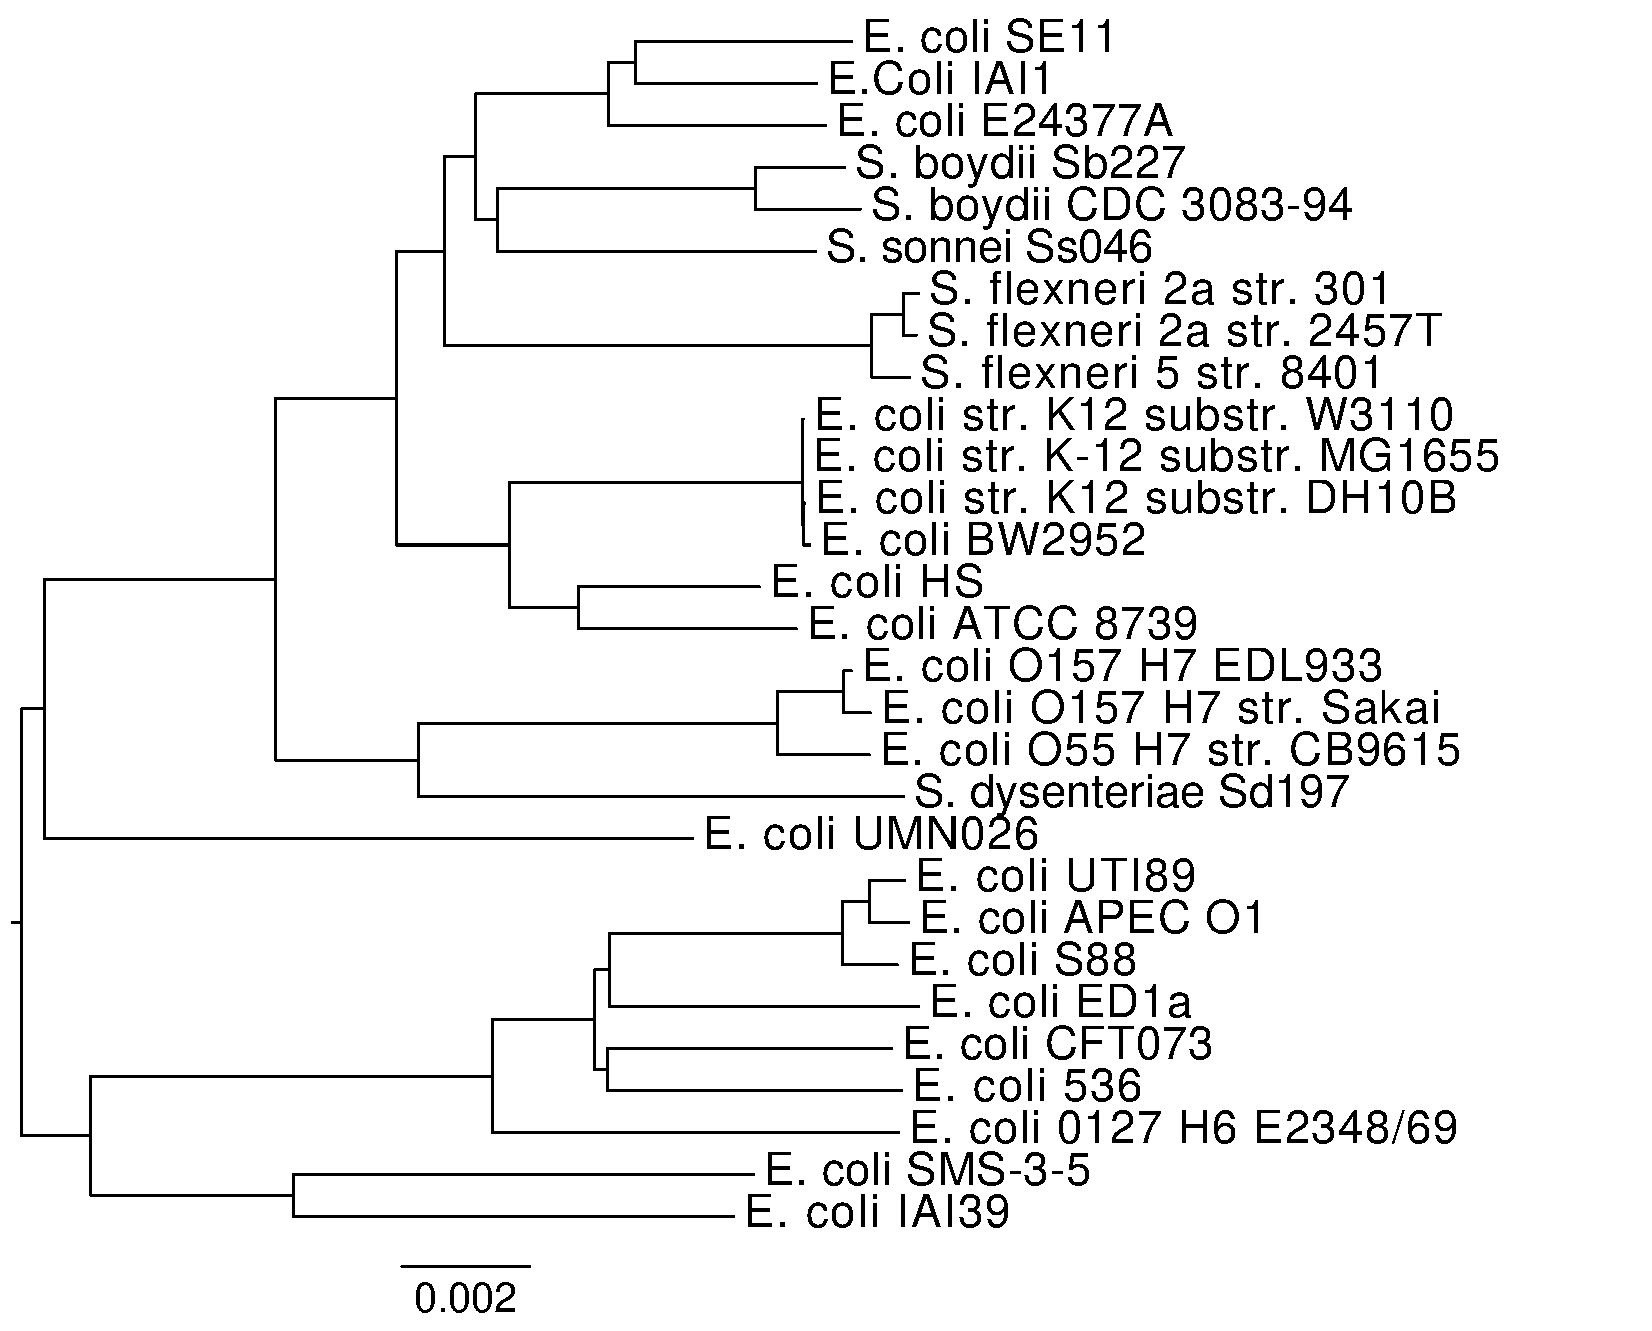
\includegraphics[width=0.99\textwidth]{img/eco29/andi_labels.pdf}
    \subcaption{\algo{andi}}
  \end{subfigure} ~
  \begin{subfigure}{0.48\textwidth}
    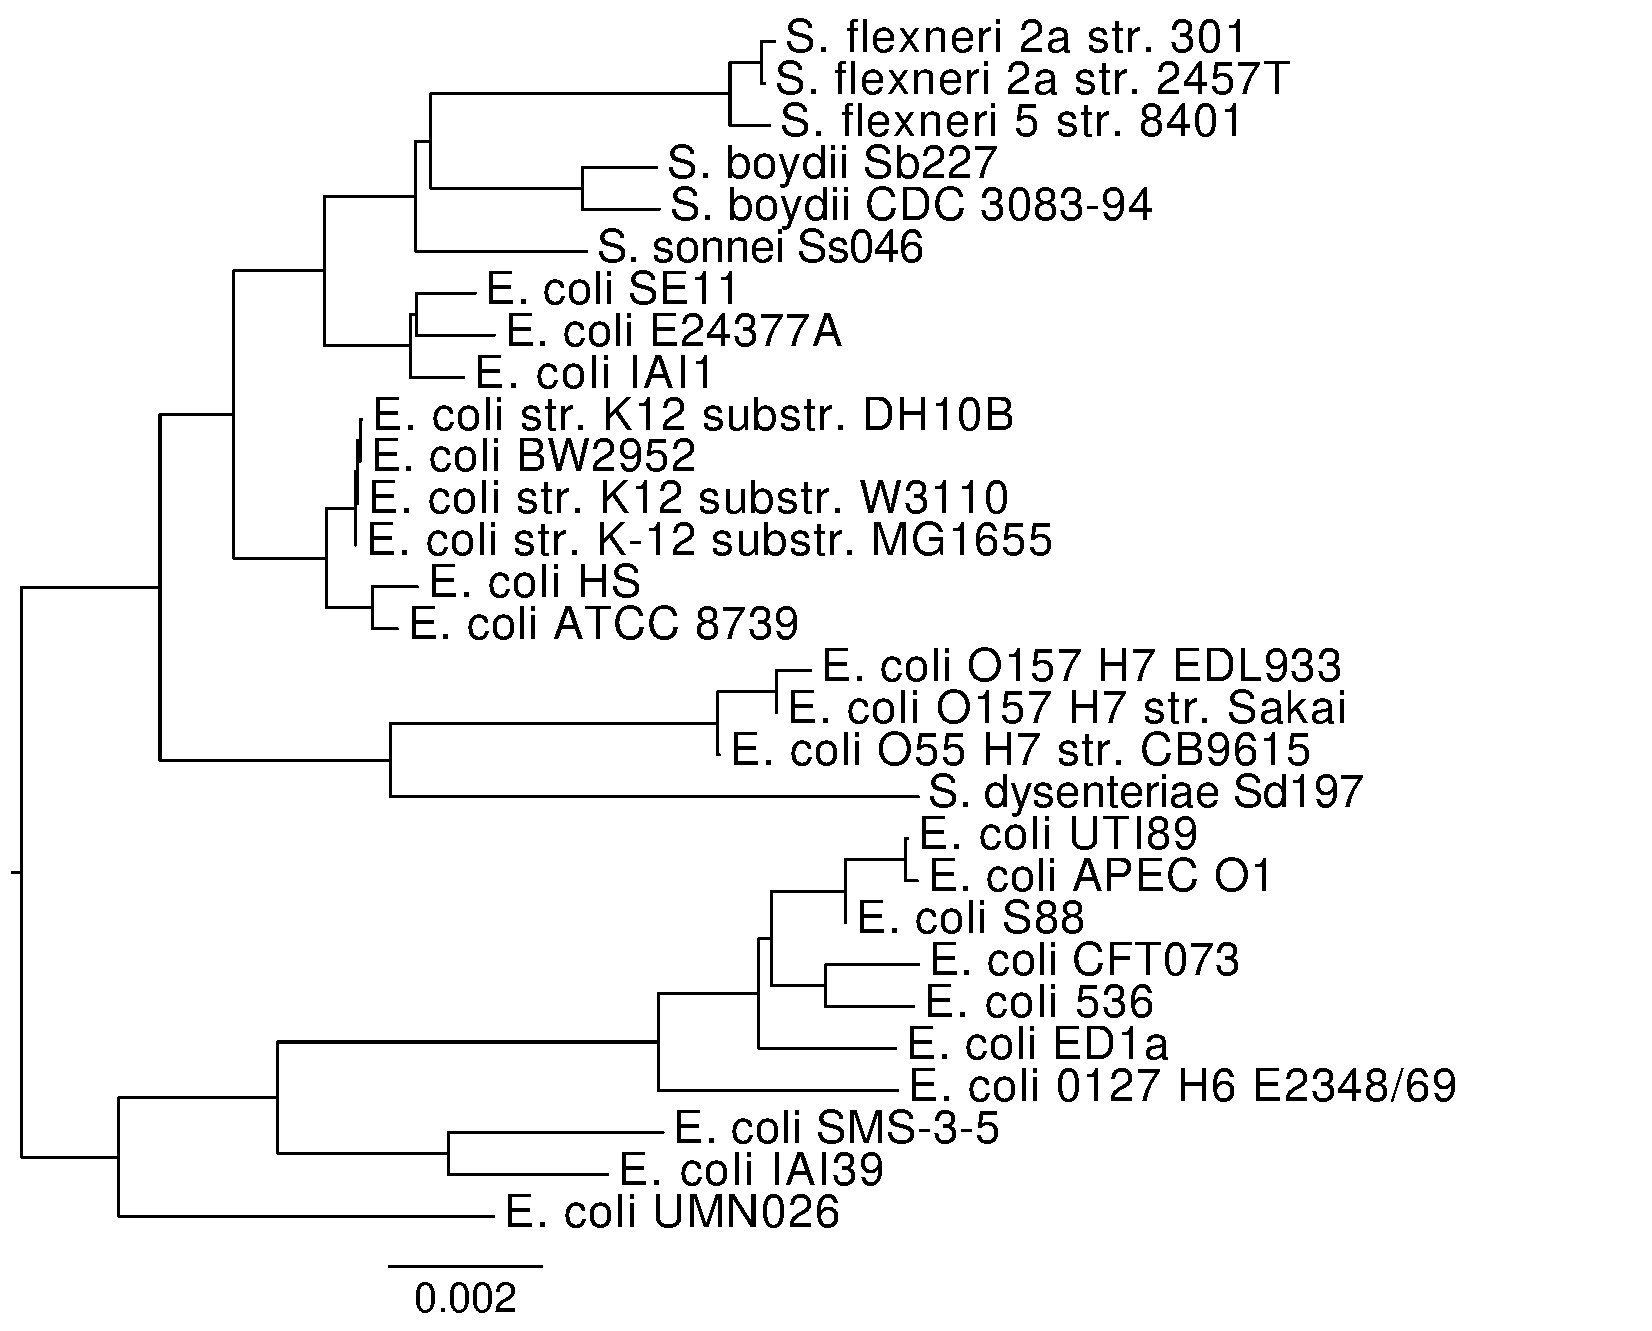
\includegraphics[width=0.99\textwidth]{img/eco29/kr_labels.pdf}
    \subcaption{\algo{kr}}
  \end{subfigure} ~
  \begin{subfigure}{0.48\textwidth}
    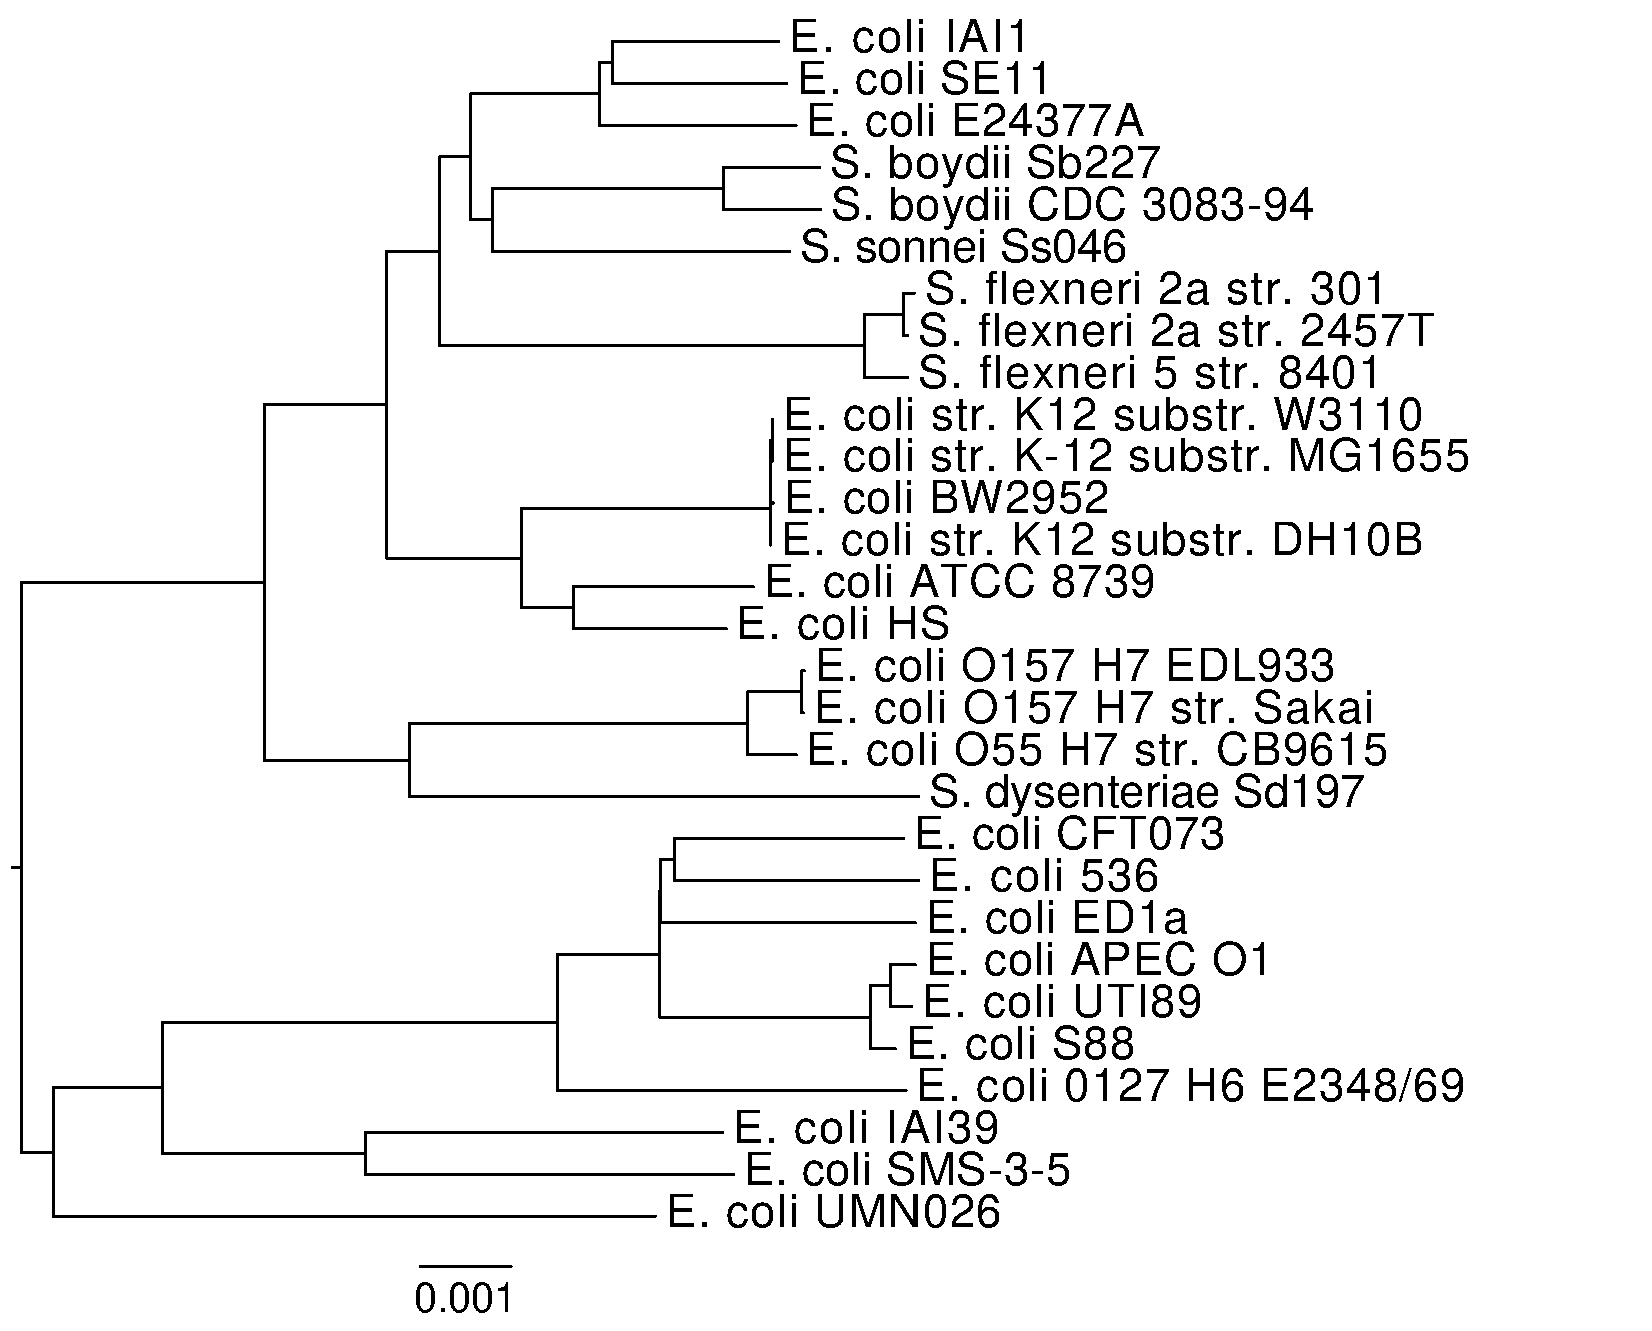
\includegraphics[width=0.99\textwidth]{img/eco29/cophylog_labels.pdf}
    \subcaption{\algo{cophylog}}
  \end{subfigure} ~
  \begin{subfigure}{0.48\textwidth}
    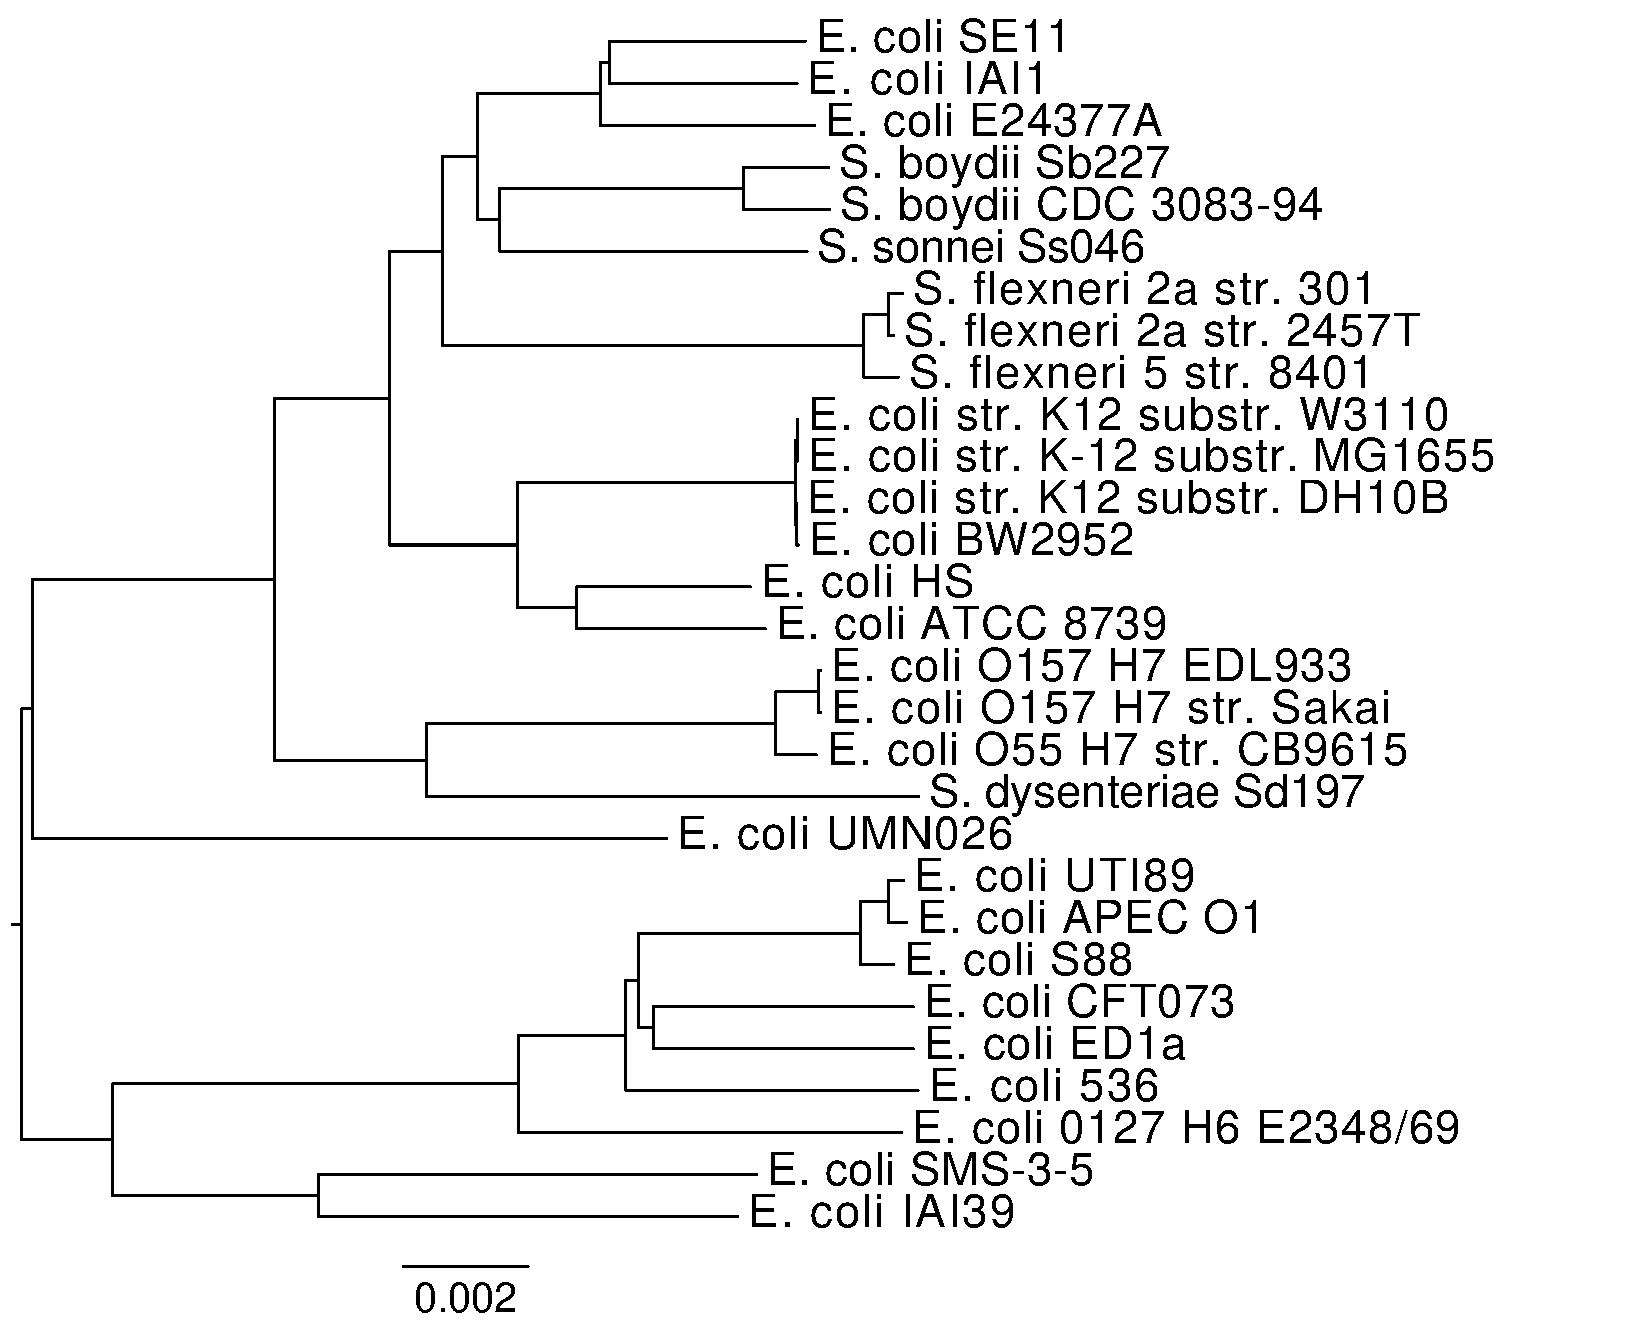
\includegraphics[width=0.99\textwidth]{img/eco29/mugsy_labels.pdf}
    \subcaption{\algo{mugsy}}
  \end{subfigure} ~
  \begin{subfigure}{0.48\textwidth}
    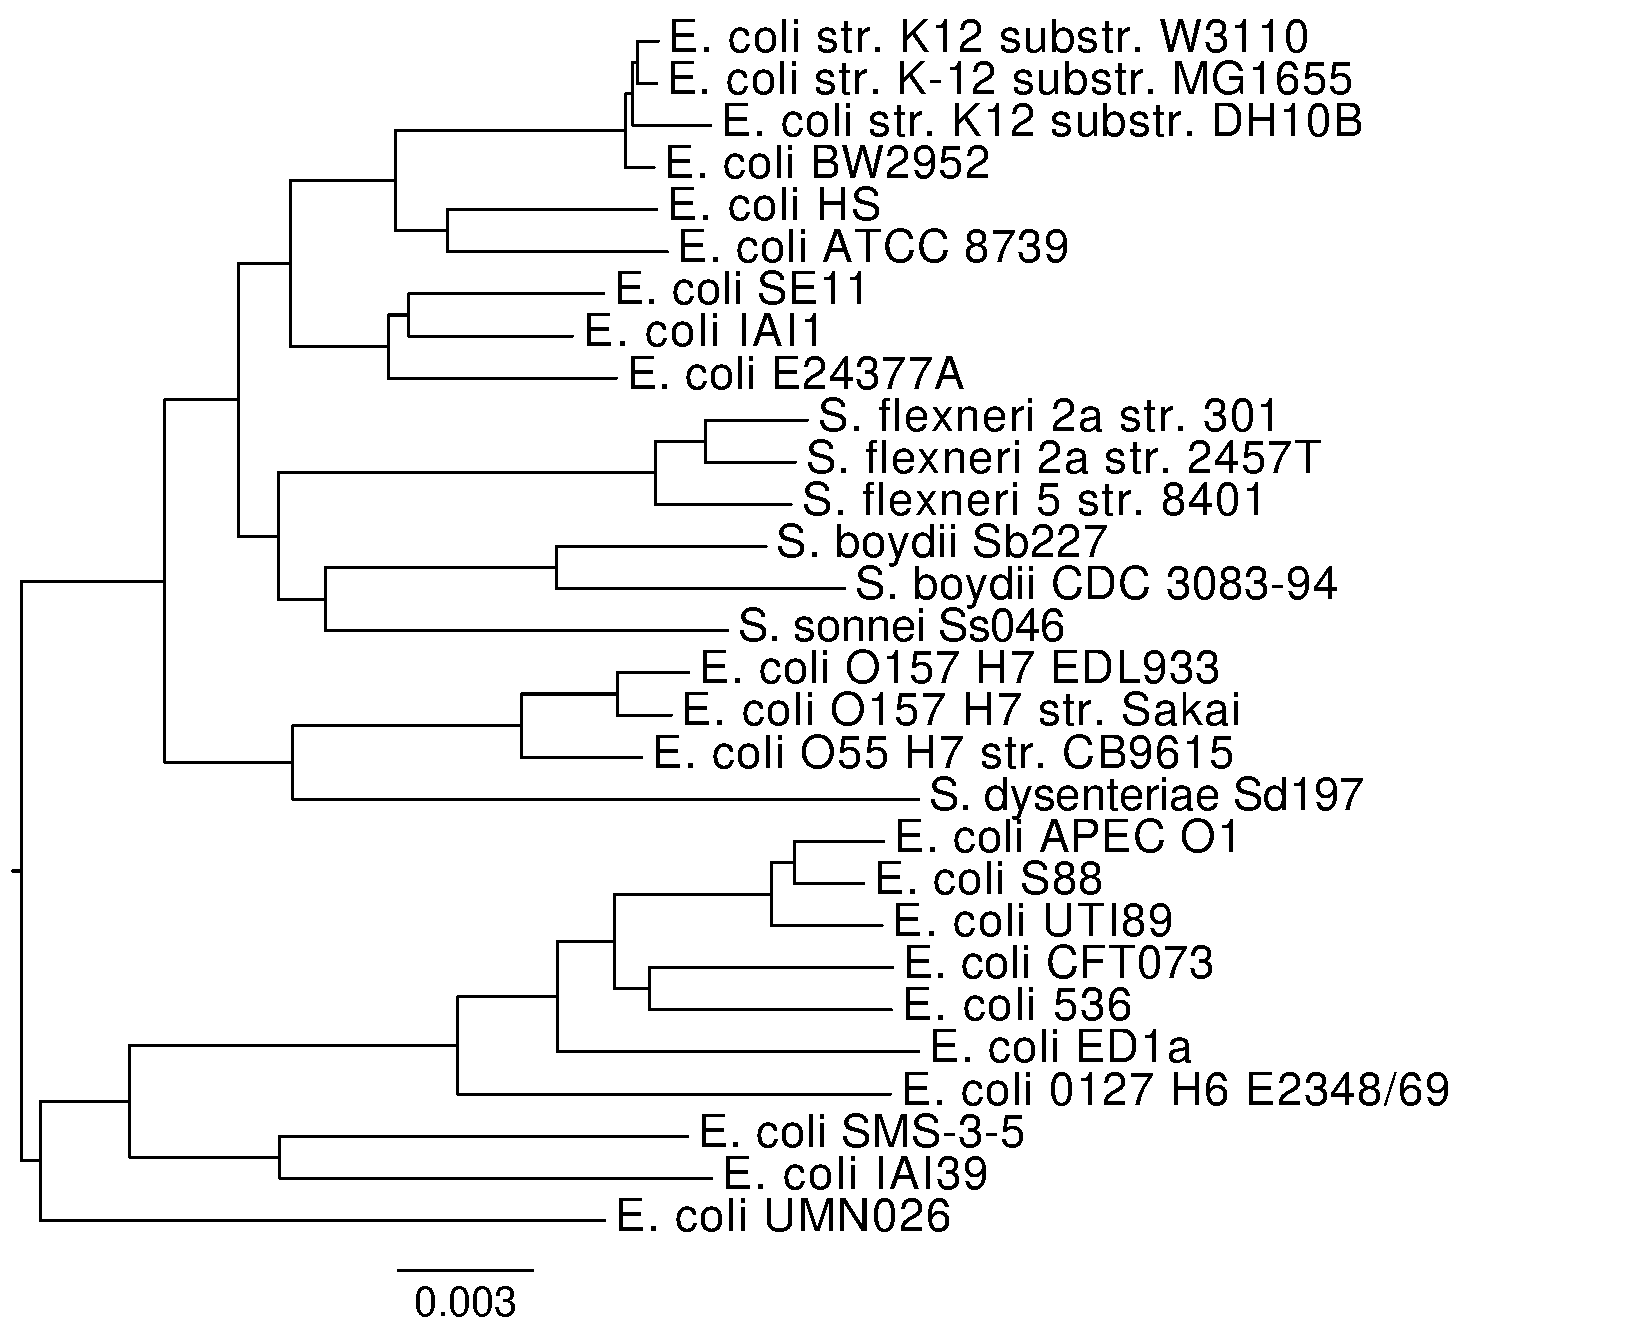
\includegraphics[width=0.99\textwidth]{img/eco29/spaced_labels.pdf}
    \subcaption{\algo{spaced}}
  \end{subfigure} ~
  \caption{\label{fig:eco29}Phylogenies for the \eco data set.}
\end{figure}

Figure~\ref{fig:eco29} shows the resulting phylogenies of four alignment-free distance measures as well as an alignment-based tree as reference. All trees were computed from the distance matrices using \algo{phylip neighbor}, \algo{retree} and drawn with \algo{figtree} \cite{figtree}.

The visually worst result is computed by \algo{kr}. A lot of its branch lengths differ noticeably from the reference tree by \algo{mugsy}. The three phylogenies by \algo{andi}, \algo{cophylog}, and \algo{mugsy} are quite similar and nearly indistinguishable. \algo{spaced} fails to cluster four \emph{E.\ Coli K12} strains together tightly.

These differences across the trees are now quantified using different metrics. First, \algo{rspr} is used to compute the topological difference between each alignment-free method and the reference tree \cite{rspr}. \andi has the smallest difference (1), followed by \algo{cophylog} (3). As expected, \algo{kr} and \algo{spaced} have the worst scores (see Table~\ref{table:eco-metrics}). The \emph{branch score} distance also takes the length of branches into account \cite{branchscore}. Thus, a smaller branch score distance means, the length of two trees are more similar. Again, the tree by \andi most closely resembles the reference, followed by \algo{cophylog}, \algo{kr}, and \algo{spaced}, in this order.

\begin{table}
  \centering
  \caption[\eco Tree Metrics]{\label{table:eco-metrics}Tree Metrics; All reported distances are with respect to \algo{mugsy}.}
  \begin{tabular}{rcccc}
    \toprule
     & \algo{andi} & \algo{kr} & \algo{cophylog} & \algo{spaced} \\\midrule
    \algo{rSPR} & 1 & 6 & 3 & 6 \\
    branch score & 0.001739 & 0.013654 &  0.009008 & 0.01415 \\
    \bottomrule
  \end{tabular}
\end{table}

The computation of the reference tree with \algo{mugsy} took $2$\,h, $49$\,min using \SI{3}{\giga\byte} of memory on machine \local. The only method needing equally much memory is \algo{kr} (see Figure~\ref{fig:eco29-resource}). But \algo{kr} is one and a half orders of magnitude faster with an average runtime of $5$\,min, $23$\,s. Thus, it is even faster than the multithreaded \algo{spaced}, using eight cores. \algo{cophylog} is slightly faster than \algo{kr}, but uses only \SI{157}{\mega\byte} of \ac{RAM}, making it the most memory-efficient tool. The fastest tool is \andi, with just \SI{100}{\second} for the sequential and \SI{27.7}{\second} for the parallel case (eight threads).

\begin{figure}
  \centering
  \includegraphics[]{img/eco29/resources-figure0.pdf}
  \caption[Resource Consumption for the \eco Test Case.]{\label{fig:eco29-resource} Resource consumption for the \eco test case. For all methods, except \algo{mugsy}, the means and variance of ten runs are shown.}
\end{figure}

\subsection*{\textit{Roseobacter}}

The genus of \emph{Roseobacter} contains highly divergent bacteria, which makes them harder to compare than \emph{E. coli}. A set of 32 \emph{Roseobacter} genomes was recently used to evaluate the results of alignment-free distance estimators for diverse genomes \cite{spaced3}. A tree based on alignments of genes was used as a reference \cite{roseo}. 

It was shown that with appropriate parameters (e.\,g.,\ $k=20$), \algo{spaced} could compute a tree with an RF-distance of 25 \cite{rfdist}, making it the most accurate method evaluated. \algo{kr} scored 46 and \algo{cophylog} 28 with $k=28$. However, with default parameters, \algo{cophylog} only achieves 39, which is worse than the 33, we measured for \andi.

The average evolutionary distance reported by \andi for the \emph{Roseobacter} genomes is one order of magnitude higher than for \eco ($0.22$ to $0.019$). At the same time, the coverage (i.\,e.,\ the amount of mapped homologous nucleotides) dropped from $0.765$ to $0.046$. This means, the result by \andi is based on only 5\% of the genome. It is interesting that 5\% of a genome suffice to gain an answer as good---or bad---as with competing methods.


\subsection*{\textit{Streptococcus pneumoniae}} \label{sec:pneu}

The largest data set used in this thesis, \pneu, contains 3085 genomes of \emph{Streptococcus pneumoniae} \cite{d3085}. Each of these genomes is given as several contigs, amounting to \SI{2.2}{\mega\basepairs} per genome and thus, \SI{6.8}{\giga\byte} for the complete data set. As all of these genomes are compared pairwise, this results in more than 4~million comparisons (9~million, if asymmetric).

It is impossible to compute distances for this data set using \algo{kr} and \algo{spaced}; both quickly exceed the available memory (\SI{256}{\giga\byte}) on machine \thymine. Thus, only the results for \andi and \algo{cophylog} can be given here. Unfortunately, no reference tree exists or can be computed via an alignment; As this data set is roughly $100$ times bigger than \eco, it needs $100^2$ times more pairwise genome comparisons. Thus, the runtime for \algo{mugsy} ($2$\,h $49$\,min) would explode to approximately $3.2$~years, which is impractical.

The figures on page~\pageref{fig:test} show the phylogenies based on the distances computed by \andi and \algo{cophylog}. The most noticeable difference is the varying scale. The average distance computed by \andi is $0.011$ and $0.0057$ for \algo{cophylog}. The RF-distance between the two trees is 4544. This may seem big, but is smaller than the average distance for two random trees of that size (6166) \cite{andi}.

It took \andi $6$\,h, $21$\,min and \SI{10}{\giga\byte} of \ac{RAM} to compute the distance matrix on \thymine with 32 threads. \algo{cophylog} is only single-threaded and ran for $36.5$~days at just \SI{2.3}{\giga\byte}. Even if \algo{cophylog} supported multi-threading, \andi still is approximately four times faster. 

\begin{figure}
  \centering
  \begin{subfigure}{0.99\textwidth}
    \centering
    \begin{overpic}[scale=0.5]{img/3085/andi_sub.pdf}
      \put(5,75){(a) \andi}
    \end{overpic}
  \end{subfigure}
  \begin{subfigure}{0.99\textwidth}
    \centering
    \begin{overpic}[scale=0.5]{img/3085/cophylog_sub.pdf}
      \put(5,75){(b) \algo{cophylog}}
    \end{overpic}
  \end{subfigure}
  \label{fig:test}
\end{figure}

\section{Further Characteristics of \andi}


\subsection{Threshold}

Recall from Section~\ref{sec:anchors} that an \emph{anchor} is a unique match of minimum length $L$. Since we are interested in anchors framing homologous regions, $L$ should be picked so that random matches are unlikely. For this, another parameter $p$ is needed, which represents the significance of an anchor pair. 

\begin{equation}
  p = 1 - P[\text{random pair}]
\end{equation}
\begin{equation}\label{eq:rand}
  P[\text{random anchor}] = \sqrt{\left(1-p\right)}
\end{equation}

The probability that an anchor was found by chance alone, in Equation~\ref{eq:rand}, depends on the length of the match. It is less likely for a long match to equal an arbitrary section in the subject than for a short match. The exact distribution of match lengths was described by \cite{kr}. For \andi, a default $p$ of $0.05$ is picked. This results in a threshold $L$ between $10$ and $16$, depending on the characteristics of the compared sequences. This is much lower than the average anchor length of $60$, depending on the chosen data set (here \textsc{eco29}, see Section~\ref{sec:eco29}). Figure~\ref{fig:threshold} displays the relationship between the threshold and the resulting distance.

\begin{figure}
  \centering
  \includegraphics[]{img/threshold/threshold-figure0.pdf}
  \caption[Threshold]{\label{fig:threshold} For each data point, ten sequence pairs with length \SI{1}{\mega\basepairs} were simulated with a distance of $0.4$. On the y-axis is the distance estimated by \andi for the specific threshold. The default $p$-value of $0.05$ equals a threshold of $15$. }
\end{figure}


\subsection{Complexity}

The requirement for fast computation of the anchor distance is low algorithmic complexity and low memory usage. Recall from Chapter~\ref{chap:alg} that computing a match to a reference \ac{ESA}, takes time $O(m \sigma)$ where $m$ is the length of the match and $\sigma$ is the size of the alphabet. For our use case, $\Sigma$ is the genomic alphabet, and hence, constant. Every nucleotide of the query is matched against the subject exactly once, leading to a runtime of $O(n)$.\footnote{W.l.o.g.\ $|S| = |Q| = n $ is assumed.} In the worst case, every nucleotide is touched again for the computation of \acp{SNP}. This still requires time $O(n)$ and $O(1)$ auxiliary working space.

The most time-consuming step is the creation of the \ac{ESA} for the subject. As shown in Chapter~\ref{chap:alg}, computing an \ac{SA}, \ac{LCP}, \ac{FVC} and \ac{RMQ} can be done in linear time, of which the \ac{SACA} takes longest, in practice. The memory requirement is $\Theta(n)$ for the \ac{ESA}.

If more than just two sequences need to be compared, multiple queries can be streamed against the same \ac{ESA}. If $k$ sequences are compared, streaming all queries against one subject takes $O(n)$ time for the \ac{ESA} construction (in theory) and $O(nk)$ time for comparison. With each sequence being a subject, computing the complete distance matrix is $O(nk^2)$ with $\Theta(n)$ working memory for the anchor distance, $O(nk)$ for the sequence data, and $O(k^2)$ for the matrix.


\subsection{Worst Case Estimations}\label{sec:worst}

The \lstinline$count_diff$ function in Listing~\ref{lst:distanchor} computes a \emph{Hamming distance}. This means it cannot detect indels. To protect against this, anchor pairs are required to be equidistant. This strategy leads to the following two problems.

\begin{figure}
  \centering
  \begin{tabular}{rccccc|ccccc|}
    & \multicolumn{5}{c}{left anchor} &  & \multicolumn{4}{c}{left anchor} \\
    \cline{2-6}\cline{8-11}
    \multicolumn{1}{r|}{$S\colon$} & \word{A} & \word{A} & \word{G} & \word{T} & \word{A} & \multicolumn{1}{c|}{\word{--}} & \word{G} & \word{C} & \wchar{T} & \wchar{T} \\
    \multicolumn{1}{r|}{$Q\colon$} & \word{A} & \word{A} & \word{G} & \word{T} & \word{A} & \multicolumn{1}{c|}{\word{A}} & \word{G} & \word{C} & \wchar{T} & \wchar{T} \\
    \cline{2-6}\cline{8-11}
  \end{tabular}
  \caption[\andi Worst Case 1]{\label{fig:worst1} This figure shows a worst case for the \emph{anchor strategy}, where anchors are found, but are not equidistant and thus, do not form a proper pair. The gap »\word{--}« does not exist in the data but is shown here for improved clarity.}
\end{figure}

In the example shown in Figure~\ref{fig:worst1}, the query contains one more character than the subject. When $d_{asym}(S,Q)$ is called, the first found anchor is \word{AAGTA}. Then the assumed substitution \wchar{A} is skipped and the second anchor is \word{GCTT}. Both anchors are unique and pass the threshold, which shall be 2, for the sake of this example. Unfortunately though, the anchors are not equidistant on both sequences and thus, no Hamming distance for the framed nucleotide(s) can be computed.

\begin{figure}
  \centering
  \begin{tabular}{rcccc|ccccc|cccc|}
    & \multicolumn{4}{c}{left anchor} & \multicolumn{5}{c}{} & \multicolumn{4}{c}{right anchor} \\
    \cline{2-5}\cline{11-14}
    \multicolumn{1}{r|}{$Q\colon$} & \wchar{A} & \wchar{A} & \wchar{G} & \wchar{T} & \wchar{C} & \wchar{T} & \wchar{A} & \wchar{--} & \wchar{T} & \wchar{T} & \wchar{A} & \wchar{A} & \wchar{G} \\ 
    \multicolumn{1}{r|}{$S\colon$} & \wchar{A} & \wchar{A} & \wchar{G} & \wchar{T} & \wchar{--} & \wchar{T} & \wchar{A} & \wchar{C} & \wchar{T} & \wchar{T} & \wchar{A} & \wchar{A} & \wchar{G} \\
    \cline{2-5}\cline{11-14}
  \end{tabular}
  \caption[\andi Worst Case 2]{\label{fig:worst2} The anchor pair frames a sequence of four nucleotides. As can be seen in the alignment, it contains two gaps. However, the Hamming distance does not see the gaps and instead counts three substitutions.}
\end{figure}

The alignment from Figure~\ref{fig:worst2} has twice the previously described problem. The middle part, framed by the two anchors, is optimally aligned using two gaps. Unfortunately, the Hamming distance counts three substitutions instead. This way, indels, which cancel themselves out, could lead to great inaccuracies. The effects of this are evaluated in Section~\ref{sec:indels}.


\subsection{Concurrency}\label{sec:concurrency}

Assume a comparison of five genome sequences. Then the calculation of $d_{asym}(1,2)$ is independent of $d_{asym}(3,2)$. So theoretically, they can be run in parallel; in fact, all comparisons for different subjects may be run in parallel. Comparisons against the same subject, however, have to await the precomputation of \ac{ESA} and end in its destruction.

At the current state of technology, multi-core processors are widely available. The number of processors $p$ per machine ranges from two for smartphones, eight for standard home computers up to 64 for servers. Even though, $p$ has been growing rapidly in the past years, it is usually still smaller than $k$.

If $p \le k$ then the computation of the distance matrix is \emph{embarrassingly parallel}. Two modes become apparent: computing multiple rows in parallel with each entry sequential or sequentially computing the entries of the rows in parallel (Figure~\ref{fig:par}). The first mode computes multiple \acp{ESA} in parallel and then streams all queries against them. Thus, it can be thought of parallelization along different subjects. This reduces the runtime to $O(nk^2/p)$, for $p < k$, at an increased memory usage of $O(nk + np + k^2)$.

\begin{figure}
  \centering
  \begin{subfigure}{0.48\textwidth}
    \centering \includegraphics[width=\textwidth]{img/concurrency/fig-concurrency-figure0.pdf}
    \subcaption{\label{fig:par-a}Parallelization along subjects}
  \end{subfigure}
  \quad
  \begin{subfigure}{0.48\textwidth}
    \centering \includegraphics[width=\textwidth]{img/concurrency/fig-concurrency-figure1.pdf}
    \subcaption{\label{fig:par-b}Parallelization along queries}
  \end{subfigure}
  \caption[Concurrency Modes]{\label{fig:par} The two subfigures show the two different possible modes of parallelization.}
\end{figure}

The second mode is algorithmically more challenging, as it requires the \ac{ESA} to be built in parallel. But its advantage is that it holds only the \ac{ESA} for a single sequence in memory, instead of $p$, and thus, it uses less memory---$O(nk + n + k^2)$---which is identical to the sequential case. The runtime is likewise reduced to $O(nk^2/p)$ in theory, where parallelization of the \ac{SACA} has the biggest impact in practice.



\todo{more copy\&paste}

\chapter{DevOps} %%%%%


\andi is written in C/C++; mostly C99 with some parts in C++11. The sources are released on \algo{GitHub} as \emph{free software} under the \textsc{Gnu General Public License version~3} \cite{GPL}. Prebundled packages using \algo{autoconf} are also available, with the latest release being {v0.9} at the time of writing.

To prove correctness even under exceptional circumstances, the code was statically analyzed by the \algo{scan-build} utility from the \algo{LLVM} framework \cite{LLVM}. 

\section{Code Documentation}

\emph{Every} function in \andi is documented using \algo{doxygen} style comments. To create the documentation run \lstinline$make code-docs$ in the main directory. You will then find the documentation under \lstinline$./docs$, duh.


\section{Unit Tests}

The unit tests achieve a coverage of more than $80\%$. They are located in the \andi repository under the \lstinline$./test$ directory. Because they require \algo{glib2}, and a C++11 compiler, they are deactivated by default. To enable them, execute

\begin{lstlisting}
~/andi %   ./configure --enable-unit-tests
\end{lstlisting}

\noindent during the installation process. You can then verify the build via 

\begin{lstlisting}
~/andi %   make check
\end{lstlisting}

\noindent The unit tests are also checked each time a commit is send to the official repository. This is done via \algo{TravisCI}.\footnote{\url{https://travis-ci.org/EvolBioInf/andi}} Thus, a warning is produced, when the builds fail, or the unit tests to not run successfully. Currently, the unit tests cover more than 80\% of the code. This is computed via the \algo{Travis} builds and a service called \algo{Coveralls}.\footnote{\url{https://coveralls.io/r/EvolBioInf/andi}}

\section{Known Issues}

These minor issues are known. I will fix them, when I have time.

\begin{enumerate}
  \item Stripping the filename from its path in join mode will not work properly on Windows because of the different path separator.
  \item I currently do not check for integer multiplication overflows in mallocs. To fix this, I might be using \lstinline$reallocarray$ from BSD.
\end{enumerate}


\section{Creating a Release}

A release should be a stable version of \andi with significant improvements over the last version. For bug fixes, dotdot release may be used.

%\subsection{Preparing a new Release}

Once \andi is matured, the new features implemented, and all tests were run, a new release can be created. First, bump the version number in \lstinline$configure.ac$. Commit that change in git, and tag this commit with \lstinline$vX.y$. Create another commit, where you set the version number to the next release (e.\,g., \lstinline$vX.z-beta$). This assures, there is only one commit and build with that specific version. Now return to the previous commit \lstinline$git checkout vX.y$.

Assert that \andi is ready for packaging with \algo{autoconf}.

\begin{lstlisting}
~ % make distcheck
make  dist-gzip am__post_remove_distdir='@:'
make[1]: Entering directory `/home/kloetzl/Projects/andi'
if test -d "andi-0.9.1-beta"; then find "andi-0.9.1-beta" -type d ! -perm -200 -exec chmod u+w {} ';' && rm -rf "andi-0.9.1-beta" || { sleep 5 && rm -rf "andi-0.9.1-beta"; }; else :; fi
test -d "andi-0.9.1-beta" || mkdir "andi-0.9.1-beta"
 (cd src && make  top_distdir=../andi-0.9.1-beta distdir=../andi-0.9.1-beta/src \
     am__remove_distdir=: am__skip_length_check=: am__skip_mode_fix=: distdir)

... Loads of output ...

=================================================
andi-0.9.1-beta archives ready for distribution: 
andi-0.9.1-beta.tar.gz
=================================================
\end{lstlisting}

If the command does not successfully builds, no tarballs will be created. This is when you really have to dive into the internals of \algo{autoconf} and \algo{automake}. Good luck with that!

% \chapter{Troubleshooting}
% \label{sec:trouble}

% No unexpected errors or bugs were reported, yet. Please contact the author in the case of exceptions.

\chapter{Notation}
%\addcontentsline{toc}{Section}{Acronyms}
\todo{Cleanup}
\begin{acronym}[SA]
  \setlength{\itemsep}{-\parsep}
  \acro{SA}{suffix array}
  \acro{SACA}{suffix array construction algorithm}
  \acro{LCP}{longest common prefix}
  \acro{ESA}{enhanced suffix array}
  \acro{CSA}{compressed suffix array}
  \acro{DNA}{deoxyribonucleic acid}
  \acro{SNP}{single nucleotide polymorphism}
  \acro{RMQ}{range minimum query}
  \acro{FVC}{first variant character}
  \acro{CPU}{central processing unit}
  \acro{GPU}{graphics processing unit}
  \acro{RAM}{random access memory}
  \acro{PRAM}{parallel random access memory}
  \acro{CREW}{concurrent read exclusive write}
  \acro{CLD}{child array}
\end{acronym}


\end{document}
